% Memoria breve (3 caras, doble columna) — plantilla uc3mmaster.
% Compilar desde esta carpeta:  latexmk -pdf memoria.tex
% Cifras: ../numeros.tex; filas de tablas: ../tablas.tex (ambos generados por ../analisis.py); figuras: ../figuras/.
\documentclass[memoria,twocolumn]{uc3mmaster}
\newgeometry{top=1.7cm,bottom=1.6cm,left=1.45cm,right=1.45cm,headheight=13pt,headsep=8pt,footskip=16pt}
\setlength{\columnsep}{0.6cm}
\usepackage{multirow}
\usetikzlibrary{arrows.meta,positioning}
\definecolor{azulm}{HTML}{2E6DB4}\definecolor{naranjam}{HTML}{D9731A}
\definecolor{verdem}{HTML}{2F9467}\definecolor{grism}{HTML}{5A6772}
% Generado por analisis.py: NO editar a mano.
\newcommand{\nDatasets}{12}
\newcommand{\nParticiones}{5}
\newcommand{\nCasos}{60}
\newcommand{\relRL}{0{,}96}
\newcommand{\cambioRL}{$-$4{,}4\,\%}
\newcommand{\casosRL}{36/60}
\newcommand{\dsRL}{7/12}
\newcommand{\pRL}{$1{,}000$}
\newcommand{\cambioVsEstRL}{$-$2{,}6\,\%}
\newcommand{\dsVsEstRL}{6/12}
\newcommand{\pVsEstRL}{$1{,}000$}
\newcommand{\peorDsRL}{$+$20{,}9\,\%}
\newcommand{\relKNN}{0{,}76}
\newcommand{\cambioKNN}{$-$24{,}3\,\%}
\newcommand{\casosKNN}{56/60}
\newcommand{\dsKNN}{12/12}
\newcommand{\pKNN}{$0{,}004$}
\newcommand{\cambioVsEstKNN}{$-$13{,}6\,\%}
\newcommand{\dsVsEstKNN}{10/12}
\newcommand{\pVsEstKNN}{$0{,}048$}
\newcommand{\peorDsKNN}{$-$0{,}4\,\%}
\newcommand{\relArbol}{1{,}00}
\newcommand{\cambioArbol}{$+$0{,}1\,\%}
\newcommand{\casosArbol}{34/60}
\newcommand{\dsArbol}{7/12}
\newcommand{\pArbol}{$1{,}000$}
\newcommand{\cambioVsEstArbol}{$+$0{,}1\,\%}
\newcommand{\dsVsEstArbol}{7/12}
\newcommand{\pVsEstArbol}{$1{,}000$}
\newcommand{\peorDsArbol}{$+$5{,}0\,\%}
\newcommand{\relRF}{1{,}00}
\newcommand{\cambioRF}{$+$0{,}5\,\%}
\newcommand{\casosRF}{27/60}
\newcommand{\dsRF}{5/12}
\newcommand{\pRF}{$1{,}000$}
\newcommand{\cambioVsEstRF}{$+$0{,}5\,\%}
\newcommand{\dsVsEstRF}{5/12}
\newcommand{\pVsEstRF}{$1{,}000$}
\newcommand{\peorDsRF}{$+$4{,}1\,\%}
\newcommand{\cambioSintRL}{$-$1{,}3\,\%}
\newcommand{\pSintRL}{$0{,}705$}
\newcommand{\dsSintRL}{7/12}
\newcommand{\relSintRL}{0{,}99}
\newcommand{\cambioSintKNN}{$-$0{,}3\,\%}
\newcommand{\pSintKNN}{$0{,}705$}
\newcommand{\dsSintKNN}{7/12}
\newcommand{\relSintKNN}{1{,}00}
\newcommand{\cambioSintArbol}{$+$0{,}3\,\%}
\newcommand{\pSintArbol}{$1{,}000$}
\newcommand{\dsSintArbol}{7/12}
\newcommand{\relSintArbol}{1{,}00}
\newcommand{\cambioSintRF}{$-$0{,}1\,\%}
\newcommand{\pSintRF}{$1{,}000$}
\newcommand{\dsSintRF}{7/12}
\newcommand{\relSintRF}{1{,}00}
\newcommand{\cambioRedRL}{$+$1{,}8\,\%}
\newcommand{\pRedRL}{$0{,}380$}
\newcommand{\dsRedRL}{5/12}
\newcommand{\relRedRL}{1{,}02}
\newcommand{\cambioRedKNN}{$+$1{,}0\,\%}
\newcommand{\pRedKNN}{$0{,}330$}
\newcommand{\dsRedKNN}{4/12}
\newcommand{\relRedKNN}{1{,}01}
\newcommand{\cambioRedArbol}{$+$1{,}4\,\%}
\newcommand{\pRedArbol}{$0{,}330$}
\newcommand{\dsRedArbol}{3/12}
\newcommand{\relRedArbol}{1{,}01}
\newcommand{\cambioRedRF}{$+$2{,}8\,\%}
\newcommand{\pRedRF}{$0{,}049$}
\newcommand{\dsRedRF}{1/12}
\newcommand{\relRedRF}{1{,}03}
\newcommand{\dimMedia}{83\,\%}
\newcommand{\fracEliminados}{22\,\%}
\newcommand{\dimMin}{38\,\%}
\newcommand{\dimMax}{92\,\%}
\newcommand{\mMedia}{0{,}4}
\newcommand{\fracConSintesis}{25\,\%}
\newcommand{\tauMediana}{0{,}18}
\newcommand{\casosNmenosUno}{38/60}
\newcommand{\wLat}{2{,}91}
\newcommand{\wLon}{2{,}85}
\newcommand{\wPop}{0{,}03}
\newcommand{\wInc}{0{,}41}
\newcommand{\fracApagados}{10\,\%}
\newcommand{\nCompCasos}{60}
\newcommand{\compMLKRRL}{$-$1{,}8\,\%}
\newcommand{\compMLKRKNN}{$-$22{,}5\,\%}
\newcommand{\compMLKRArbol}{$+$2{,}0\,\%}
\newcommand{\compMLKRRF}{$+$2{,}6\,\%}
\newcommand{\rangoMLKR}{5{,}7}
\newcommand{\compPGRL}{$-$15{,}7\,\%}
\newcommand{\compPGKNN}{$-$18{,}0\,\%}
\newcommand{\compPGArbol}{$+$0{,}7\,\%}
\newcommand{\compPGRF}{$+$0{,}8\,\%}
\newcommand{\rangoPG}{4{,}6}
\newcommand{\compYJMVRL}{$+$2{,}4\,\%}
\newcommand{\compYJMVKNN}{$-$14{,}5\,\%}
\newcommand{\compYJMVArbol}{$+$1{,}5\,\%}
\newcommand{\compYJMVRF}{$+$1{,}7\,\%}
\newcommand{\rangoYJMV}{5{,}0}
\newcommand{\compCuantRL}{$+$8{,}1\,\%}
\newcommand{\compCuantKNN}{$-$11{,}8\,\%}
\newcommand{\compCuantArbol}{$+$0{,}1\,\%}
\newcommand{\compCuantRF}{$+$0{,}0\,\%}
\newcommand{\rangoCuant}{6{,}4}
\newcommand{\compEstPCARL}{$-$1{,}8\,\%}
\newcommand{\compEstPCAKNN}{$-$12{,}4\,\%}
\newcommand{\compEstPCAArbol}{$-$0{,}6\,\%}
\newcommand{\compEstPCARF}{$-$1{,}9\,\%}
\newcommand{\rangoEstPCA}{4{,}6}
\newcommand{\compPCAnoventaRL}{$+$0{,}6\,\%}
\newcommand{\compPCAnoventaKNN}{$-$10{,}4\,\%}
\newcommand{\compPCAnoventaArbol}{$+$19{,}3\,\%}
\newcommand{\compPCAnoventaRF}{$+$17{,}9\,\%}
\newcommand{\rangoPCAnoventa}{8{,}1}
\newcommand{\compPCAcvRL}{$-$1{,}0\,\%}
\newcommand{\compPCAcvKNN}{$-$12{,}0\,\%}
\newcommand{\compPCAcvArbol}{$+$18{,}7\,\%}
\newcommand{\compPCAcvRF}{$+$15{,}1\,\%}
\newcommand{\rangoPCAcv}{7{,}4}
\newcommand{\compPsrRL}{$-$6{,}1\,\%}
\newcommand{\compPsrKNN}{$-$25{,}0\,\%}
\newcommand{\compPsrArbol}{$-$1{,}1\,\%}
\newcommand{\compPsrRF}{$-$2{,}3\,\%}
\newcommand{\rangoPsr}{3{,}2}
\newcommand{\compPRL}{$-$4{,}4\,\%}
\newcommand{\compPKNN}{$-$24{,}3\,\%}
\newcommand{\compPArbol}{$+$0{,}1\,\%}
\newcommand{\compPRF}{$+$0{,}5\,\%}
\newcommand{\rangoP}{4{,}7}
\newcommand{\mejorAlt}{estándar + PCA}
\newcommand{\rangoMejorAlt}{4{,}6}
\newcommand{\nReps}{10}
\newcommand{\vMedia}{0{,}80}
\newcommand{\vFracUno}{22\,\%}
\newcommand{\nSintMedia}{3{,}9}
\newcommand{\ctrlIniAleat}{$+$0{,}6\,\%}
\newcommand{\pCtrlIniAleat}{$1{,}000$}
\newcommand{\ctrlIniAleatRL}{$+$1{,}7\,\%}
\newcommand{\ctrlSigmaBajo}{$+$0{,}5\,\%}
\newcommand{\pCtrlSigmaBajo}{$1{,}000$}
\newcommand{\ctrlSigmaBajoRL}{$-$0{,}1\,\%}
\newcommand{\ctrlSigmaAlto}{$+$0{,}9\,\%}
\newcommand{\pCtrlSigmaAlto}{$1{,}000$}
\newcommand{\ctrlSigmaAltoRL}{$-$0{,}4\,\%}
\newcommand{\ctrlPobDoble}{$+$0{,}2\,\%}
\newcommand{\pCtrlPobDoble}{$1{,}000$}
\newcommand{\ctrlPobDobleRL}{$-$0{,}2\,\%}
\newcommand{\nAblCasos}{24}
\newcommand{\ctrlPesos}{$+$2{,}2\,\%}
\newcommand{\ctrlPesosRL}{$+$6{,}5\,\%}
\newcommand{\pCtrlPesos}{$0{,}424$}
\newcommand{\ctrlExp}{$+$10{,}0\,\%}
\newcommand{\ctrlExpRL}{$+$2{,}2\,\%}
\newcommand{\pCtrlExp}{$0{,}012$}
\newcommand{\ctrlAleat}{$+$6{,}2\,\%}
\newcommand{\ctrlAleatRL}{$+$3{,}0\,\%}
\newcommand{\pCtrlAleat}{$0{,}012$}
\newcommand{\ctrlMI}{$+$14{,}9\,\%}
\newcommand{\ctrlMIRL}{$+$6{,}8\,\%}
\newcommand{\pCtrlMI}{$0{,}012$}
\newcommand{\ctrlYJMI}{$+$11{,}0\,\%}
\newcommand{\ctrlYJMIRL}{$+$10{,}3\,\%}
\newcommand{\pCtrlYJMI}{$0{,}014$}
\newcommand{\nCtrlCasos}{24}
\newcommand{\rangoCeroR}{$+$2{,}2\,\%}
\newcommand{\pRangoCero}{$1{,}000$}
\newcommand{\dsPeorRangoCero}{7}
\newcommand{\rangoUnoR}{$+$0{,}3\,\%}
\newcommand{\pRangoUno}{$1{,}000$}
\newcommand{\dsPeorRangoUno}{6}
\newcommand{\rangoCuatroR}{$+$0{,}5\,\%}
\newcommand{\pRangoCuatro}{$1{,}000$}
\newcommand{\dsPeorRangoCuatro}{7}
\newcommand{\rangoOchoR}{$+$1{,}7\,\%}
\newcommand{\pRangoOcho}{$0{,}256$}
\newcommand{\dsPeorRangoOcho}{9}
\newcommand{\bordeUno}{11\,\%}
\newcommand{\bordeDos}{7\,\%}
\newcommand{\bordeCuatro}{8\,\%}
\newcommand{\bordeOcho}{5\,\%}
\newcommand{\nRango}{24}
\newcommand{\mleFueraDos}{24\,\%}
\newcommand{\nAlgCasos}{24}
\newcommand{\rangoCMA}{1{,}9}
\newcommand{\algMejor}{CMA-ES}
\newcommand{\algKNNcma}{$-$25{,}7\,\%}
\newcommand{\algKNNaleat}{$-$21{,}0\,\%}
\newcommand{\algKNNmin}{$-$24{,}8\,\%}
\newcommand{\algKNNmax}{$-$23{,}3\,\%}
\newcommand{\segMediana}{191}
\newcommand{\segMax}{243}
\newcommand{\msPorEval}{191}
\newcommand{\segMLKR}{16{,}8}
\newcommand{\segPG}{6{,}1}
\newcommand{\segYJMV}{0{,}6}
\newcommand{\popMin}{11}
\newcommand{\popMax}{13}
\newcommand{\muMin}{5}
\newcommand{\muMax}{6}
\newcommand{\muEffMin}{3{,}4}
\newcommand{\muEffMax}{4{,}0}
\newcommand{\genMin}{77}
\newcommand{\genMax}{91}
\newcommand{\nParadaPresupuesto}{12}
\newcommand{\nParadaTotal}{12}
\newcommand{\evalMejorMediana}{971}
\newcommand{\evalMejorMin}{658}
\newcommand{\mejoraFitnessMediana}{$-$12{,}1\,\%}
\newcommand{\sigmaFinMin}{0{,}007}
\newcommand{\sigmaFinMax}{0{,}06}
\newcommand{\cribSelRL}{$-$2{,}5\,\%}
\newcommand{\cribSelKNN}{$-$23{,}9\,\%}
\newcommand{\cribSelArbol}{$+$0{,}1\,\%}
\newcommand{\cribSelRF}{$+$0{,}8\,\%}
\newcommand{\cribDimSel}{72\,\%}
\newcommand{\cribFijoRL}{$-$5{,}4\,\%}
\newcommand{\cribFijoKNN}{$-$25{,}0\,\%}
\newcommand{\cribFijoArbol}{$-$0{,}5\,\%}
\newcommand{\cribFijoRF}{$+$0{,}0\,\%}
\newcommand{\cribDimFijo}{89\,\%}
\newcommand{\cribPcaRL}{$-$2{,}7\,\%}
\newcommand{\cribPcaKNN}{$-$23{,}9\,\%}
\newcommand{\cribPcaArbol}{$+$0{,}8\,\%}
\newcommand{\cribPcaRF}{$+$1{,}9\,\%}
\newcommand{\cribDimPca}{70\,\%}
\newcommand{\cribFijoNoReduce}{27/60}
% Generado por analisis.py: filas de las tablas (una macro por tabla).
\newcommand{\filasPrincipal}{%
R. lineal & 0{,}98 & 0{,}94 & \textbf{0{,}96} & 7/12 & $1{,}000$ & $-$2{,}6\,\%\\
KNN & 0{,}88 & 0{,}75 & \textbf{0{,}76} & 12/12 & $0{,}004$ & $-$13{,}6\,\%\\
Árbol & 1{,}00 & 0{,}99 & \textbf{1{,}00} & 7/12 & $1{,}000$ & $+$0{,}1\,\%\\
RF & 1{,}00 & 0{,}98 & \textbf{1{,}00} & 5/12 & $1{,}000$ & $+$0{,}5\,\%\\
}
\newcommand{\filasDimension}{%
diabetes & 10 & 8{,}0 & 0{,}6 & 8{,}6 & 0{,}46\\
concrete & 8 & 6{,}6 & 0{,}0 & 6{,}6 & 0{,}47\\
stock & 9 & 7{,}6 & 0{,}4 & 8{,}0 & 0{,}30\\
space\_ga & 6 & 3{,}8 & 0{,}4 & 4{,}2 & 0{,}09\\
sulfur & 6 & 5{,}0 & 0{,}0 & 5{,}0 & 0{,}01\\
wine\_quality & 11 & 9{,}6 & 0{,}2 & 9{,}8 & 0{,}41\\
kin8nm & 8 & 7{,}0 & 0{,}0 & 7{,}0 & 0{,}34\\
bank8FM & 8 & 6{,}8 & 0{,}2 & 7{,}0 & 0{,}05\\
puma8NH & 8 & 2{,}2 & 2{,}4 & 4{,}6 & 1{,}83\\
house\_8L & 8 & 7{,}0 & 0{,}0 & 7{,}0 & 0{,}12\\
cpu\_small & 12 & 10{,}8 & 0{,}2 & 11{,}0 & 0{,}19\\
california & 8 & 6{,}6 & 0{,}0 & 6{,}6 & 0{,}02\\
}
\newcommand{\filasComparativa}{%
estándar & 0{,}98 & 0{,}88$^*$ & 1{,}00 & 1{,}00 & 5{,}3 & 1{,}00\\
YJ máx.\ verosimilitud & 1{,}02 & 0{,}85$^*$ & 1{,}01 & 1{,}02 & 5{,}0 & 1{,}00\\
cuantiles & 1{,}08 & 0{,}88$^*$ & 1{,}00 & 1{,}00 & 6{,}4 & 1{,}00\\
solo PCA (95\,\%) & 1{,}01 & 0{,}90$^*$ & 1{,}19$^*$ & 1{,}18$^*$ & 8{,}1 & 0{,}79\\
solo PCA (\% por VC) & 0{,}99 & 0{,}88$^*$ & 1{,}19$^*$ & 1{,}15 & 7{,}4 & 0{,}91\\
estándar + su PCA & 0{,}98 & 0{,}88$^*$ & 0{,}99 & 0{,}98 & 4{,}6 & 2{,}00\\
MLKR & 0{,}98 & 0{,}78 & 1{,}02 & 1{,}03 & 5{,}7 & 1{,}00\\
PG (gplearn) & \textbf{0{,}84} & 0{,}82$^*$ & 1{,}01 & 1{,}01 & 4{,}6 & 2{,}00\\
$P$ sin reducir & 0{,}94 & \textbf{0{,}75} & \textbf{0{,}99} & \textbf{0{,}98} & 3{,}2 & 2{,}00\\
\textbf{$P$} & 0{,}96 & 0{,}76 & 1{,}00 & 1{,}00 & 4{,}7 & 0{,}83\\
}
\newcommand{\filasAblacion}{%
\multicolumn{4}{@{}l}{\emph{Piezas}}\\
\quad solo pesos ($\lambda=1$) & $+$2{,}2\,\% & $+$6{,}5\,\% & $-$0{,}1\,\%\\
\quad solo exponentes ($w=1$) & $+$10{,}0\,\%$^*$ & $+$2{,}2\,\% & $+$0{,}4\,\%\\
\midrule
\multicolumn{4}{@{}l}{\emph{Sin búsqueda}}\\
\quad pesos por inf.\ mutua & $+$14{,}9\,\%$^*$ & $+$6{,}8\,\% & $+$3{,}6\,\%\\
\quad YJ (MV) + pesos inf.\ mutua & $+$11{,}0\,\% & $+$10{,}3\,\% & $+$3{,}6\,\%\\
\midrule
\multicolumn{4}{@{}l}{\emph{Búsqueda}}\\
\quad búsqueda aleatoria (1000 puntos) & $+$6{,}2\,\%$^*$ & $+$3{,}0\,\% & $+$2{,}0\,\%\\
\midrule
\multicolumn{4}{@{}l}{\emph{Inicio}}\\
\quad media inicial aleatoria & $+$0{,}6\,\% & $+$1{,}7\,\% & $+$0{,}6\,\%\\
\quad $\sigma_0=0{,}1$ & $+$0{,}5\,\% & $-$0{,}1\,\% & $+$0{,}8\,\%\\
\quad $\sigma_0=0{,}4$ & $+$0{,}9\,\% & $-$0{,}4\,\% & $+$0{,}6\,\%\\
\quad población $\times2$ & $+$0{,}2\,\% & $-$0{,}2\,\% & $+$1{,}3\,\%\\
\midrule
\multicolumn{4}{@{}l}{\emph{Rango}}\\
\quad $\lambda\in[-1,1]$ & $+$0{,}3\,\% & $+$1{,}5\,\% & $-$0{,}3\,\%\\
\quad $\lambda\in[-4,4]$ & $+$0{,}5\,\% & $+$1{,}4\,\% & $+$1{,}1\,\%\\
\quad $\lambda\in[-8,8]$ & $+$1{,}7\,\% & $+$5{,}0\,\% & $+$1{,}4\,\%\\
}
\newcommand{\filasControles}{%
solo pesos ($\lambda=1$) & $+$2{,}2\,\% & $+$6{,}5\,\% & $-$0{,}1\,\%\\
solo exponentes ($w=1$) & $+$10{,}0\,\%$^*$ & $+$2{,}2\,\% & $+$0{,}4\,\%\\
búsqueda aleatoria & $+$6{,}2\,\%$^*$ & $+$3{,}0\,\% & $+$2{,}0\,\%$^*$\\
pesos por inf.\ mutua & $+$14{,}9\,\%$^*$ & $+$6{,}8\,\% & $+$3{,}6\,\%\\
YJ (MV) + pesos inf.\ mutua & $+$11{,}0\,\%$^*$ & $+$10{,}3\,\% & $+$3{,}6\,\%\\
}
\newcommand{\filasAlgoritmos}{%
\textbf{CMA-ES} & 1{,}9 & $-$25{,}7\,\% & $-$7{,}7\,\%\\
AG (propio) & 2{,}8 & $-$24{,}4\,\% & $-$8{,}5\,\%\\
HS & 3{,}2 & $-$24{,}5\,\% & $-$8{,}3\,\%\\
BBO & 4{,}4 & $-$24{,}8\,\% & $-$8{,}0\,\%\\
PSO & 4{,}5 & $-$24{,}1\,\% & $-$5{,}1\,\%\\
DE & 5{,}4 & $-$23{,}3\,\% & $-$5{,}9\,\%\\
ABC & 5{,}9 & $-$24{,}0\,\% & $-$2{,}4\,\%\\
búsqueda aleatoria & 7{,}9 & $-$21{,}0\,\% & $-$4{,}9\,\%\\
}
\newcommand{\filasCoste}{%
P (CMA-ES, 1000 evaluaciones) & 190{,}6 & 242{,}6\\
MLKR & 16{,}8 & 41{,}8\\
PG (gplearn) & 6{,}1 & 14{,}1\\
PCA v-CV & 1{,}0 & 11{,}5\\
YJ máx. verosimilitud & 0{,}6 & 4{,}3\\
cuantiles & 0{,}1 & 0{,}8\\
estándar + PCA & 0{,}0 & 0{,}0\\
}
\newcommand{\filasDatasets}{%
diabetes & 442 & 10\\
concrete & 1\,030 & 8\\
stock & 950 & 9\\
space\_ga & 3\,107 & 6\\
sulfur & 10\,000 & 6\\
wine\_quality & 6\,497 & 11\\
kin8nm & 8\,192 & 8\\
bank8FM & 8\,192 & 8\\
puma8NH & 8\,192 & 8\\
house\_8L & 10\,000 & 8\\
cpu\_small & 8\,192 & 12\\
california & 20\,640 & 8\\
}


\titulo{Transformación evolutiva de atributos}
\asignatura{IA con inspiración biológica}
\autor{Andrea López Salazar}{}
\graphicspath{{../figuras/}}
\captionsetup{font=footnotesize,skip=3pt}
\setlength{\textfloatsep}{7pt plus 2pt}
\setlength{\floatsep}{5pt plus 2pt}
\setlength{\dbltextfloatsep}{7pt plus 2pt}
\titlespacing*{\section}{0pt}{0.9ex plus .3ex}{0.4ex}
\titlespacing*{\subsection}{0pt}{0.7ex plus .2ex}{0.25ex}
\setlength{\parskip}{2pt plus 1pt}

\begin{document}
\twocolumn[{%
\begin{tikzpicture}[remember picture,overlay,every node/.style={anchor=west,text=white,font=\sffamily}]
  \fill[uc3mazul] (current page.north west) rectangle ([yshift=-3.0cm]current page.north east);
  \fill[uc3mcian] ([yshift=-3.0cm]current page.north west) rectangle ([yshift=-3.1cm]current page.north east);
  \node[font=\sffamily\scriptsize\bfseries] at ([xshift=1.45cm,yshift=-0.75cm]current page.north west)
     {MEMORIA \textbullet\ IA CON INSPIRACIÓN BIOLÓGICA \textbullet\ MÁSTER EN CIENCIA Y TECNOLOGÍA \textbullet\ UC3M};
  \node[font=\sffamily\Large\bfseries] at ([xshift=1.45cm,yshift=-1.5cm]current page.north west)
     {Transformación evolutiva de atributos: forma, relevancia, reducción y síntesis};
  \node[font=\sffamily\small] at ([xshift=1.45cm,yshift=-2.35cm]current page.north west) {Andrea López Salazar};
  \node[font=\sffamily\small,anchor=east] at ([xshift=-1.45cm,yshift=-2.35cm]current page.north east)
     {Curso 2026--2027};
\end{tikzpicture}
\vspace*{1.05cm}
\begin{resultado}[Resumen]\small
Aprendemos con CMA-ES, solo con el entrenamiento, una transformación $X\!\to\!X'$ con \emph{menos} atributos que $X$:
corrige la \emph{forma} de cada atributo (Yeo-Johnson), aprende su \emph{relevancia} (pesos), \emph{elimina} los
atributos cuyo peso queda por debajo de un umbral $\tau$ que aprende la propia evolución y \emph{sintetiza}
componentes principales del espacio aprendido sin pasar de $n-1$ atributos. En \nDatasets{} datasets $\times$
\nParticiones{} particiones no usadas para diseñarla, $X'$ usa de media el \dimMedia{} de los atributos (nunca $n$) y
el error baja de forma concluyente en KNN (\cambioKNN, \dsKNN{} datasets) y, sin significación, en regresión lineal
(\cambioRL); en los árboles queda igual (\cambioArbol, RF \cambioRF). Reducir cuesta poco frente a la versión sin
reducir ($2n$ atributos) salvo en Random Forest (\cambioRedRF), que pierde las direcciones oblicuas que la síntesis le
daba: con $\dim X'<n$ la síntesis y la reducción compiten. Entre las transformaciones que no aumentan la dimensión,
$P$ tiene el mejor rango medio.
\end{resultado}
\vspace{1pt}}]

\section{Problema y método}
El enunciado pide un programa $P$ que, viendo solo $(X_t,y_t)$, haga \textbf{síntesis y reducción de la
dimensionalidad} ($\dim X'<n$, con un criterio de eliminación que dependa del algoritmo evolutivo) y consiga que un
modelo \emph{arbitrario} $M$ entrenado con $X'_t$ tenga menor MAE en validación que con $X_t$ ($e'<e$). Cada familia
de modelos es sensible a cosas distintas: KNN a la geometría, la regresión lineal (RL) a la forma de cada atributo y
los árboles solo a las \emph{direcciones} por las que pueden cortar (son invariantes a cualquier cambio monótono por
atributo). $P$ se construye por bloques (Fig.~\ref{fig:esquema}): \textbf{(1) forma}, Yeo-Johnson con
$\lambda_j\in[-2,2]$; \textbf{(2) relevancia}, estandarizar y multiplicar por $w_j\in[0,3]$; \textbf{(3) reducción},
se conservan solo los atributos $S=\{j:w_j\ge\tau\}$; \textbf{(4) síntesis}, se añaden las $m$ primeras componentes
principales $p=V_m^\top(z_S-\bar z_S)$ del espacio aprendido, con $m=\mathrm{round}(\rho\,(n-1-|S|))$.

\begin{figure}[t]
\centering\def\esquemaescala{0.66}
% Esquema del método P, compartido por memoria, paper y póster.
% Requiere: tikz con las librerías arrows.meta y positioning; colores azulm, naranjam, verdem, grism.
% \esquemaescala permite reducirlo o ampliarlo sin tocar el dibujo.
\providecommand{\esquemaescala}{1}
\begin{tikzpicture}[scale=\esquemaescala, every node/.style={transform shape},
  node distance=3.5mm and 3.5mm,
  caja/.style={draw=azulm, rounded corners=2pt, fill=azulm!8, align=center, inner sep=2.5pt,
               minimum height=9mm, font=\footnotesize},
  sint/.style={caja, draw=verdem, fill=verdem!10},
  red/.style={caja, draw=naranjam, fill=naranjam!8},
  fl/.style={-{Stealth[length=2mm]}, thick, azulm!80!black},
  fv/.style={fl, verdem!80!black},
  fn/.style={fl, naranjam!80!black}]
% fila 1: bloques por atributo (forma, escala, relevancia)
\node (x) {$x_j$};
\node[caja, right=of x]   (yj) {1. Forma\\$\psi(x_j;\lambda_j)$};
\node[caja, right=of yj]  (st) {Escala\\$(\psi_j-\mu_j)/\sigma_j$};
\node[caja, right=of st]  (w)  {2. Relevancia\\$\times\,w_j$};
\node[right=of w] (z) {$z_j$};
\draw[fl] (x)--(yj); \draw[fl] (yj)--(st); \draw[fl] (st)--(w); \draw[fl] (w)--(z);
% fila 2: reducción, síntesis y salida
\node[red, below=7mm of st] (sel) {3. Reducción\\$S=\{j: w_j\ge\tau\}$};
\node[sint, right=5mm of sel] (pca) {4. Síntesis\\$p_{1..m}=V_m^{\top}(z_S-\bar z_S)$};
\node[draw=grism, thick, rounded corners=2pt, fill=white, font=\footnotesize, minimum height=7mm, align=center,
     below=5mm of pca] (xp) {$X'=[\,z_S\;|\;p_1\ldots p_m\,]$,\; $|S|+m\le n-1$};
\draw[fn] (z.south) |- ([yshift=3.5mm]sel.north) -- (sel.north);
\draw[fv] (sel.east) -- (pca.west);
\draw[fv] (pca.south) -- (xp.north);
\draw[fn] (sel.south) |- (xp.west);
\node[font=\scriptsize\itshape, text=grism, align=right, anchor=east] at ([xshift=-3mm]sel.west)
     {si $|S|=n$, fuera\\el de menor $w_j$};
\node[font=\scriptsize\itshape, text=grism, align=left, anchor=west] at ([xshift=2mm]pca.east)
     {$m=\mathrm{round}(\rho\,(n{-}1{-}|S|))$};
% búsqueda
\node[caja, draw=naranjam, fill=naranjam!10, above=6mm of st, align=center] (cma)
     {CMA-ES busca $\theta=(\lambda,w,\tau,\rho)$:\; $\lambda_j\in[-2,2]$,\; $w_j,\tau\in[0,3]$,\; $\rho\in[0,1]$\\
      minimizando el MAE de validación cruzada de KNN en el entrenamiento};
\draw[fn] (cma.south -| yj) -- (yj.north);
\draw[fn] (cma.south -| w) -- (w.north);
\end{tikzpicture}

\caption{El programa $P$. CMA-ES aprende forma, relevancia, el umbral de eliminación $\tau$ y la fracción de síntesis
$\rho$; la decodificación garantiza $\dim X'\le n-1$.}
\label{fig:esquema}
\end{figure}

\textbf{El criterio de eliminación es evolutivo.} El individuo es $\theta=(\lambda,w,\tau,\rho)$, con $2n+2$ genes
reales: CMA-ES decide \emph{qué} atributos se van (los de menor peso) y \emph{cuántos} (el umbral $\tau\in[0,3]$).
La restricción $\dim X'<n$ está en la decodificación: si ningún peso cae bajo $\tau$ se elimina el de menor peso, así
que todo individuo es válido y no hay que reparar ni descartar. No añadimos penalización por dimensión: quitar más
atributos solo compensa si mejora el fitness, y así no hay hiperparámetros nuevos que ajustar.
\textbf{Fitness}: MAE de validación cruzada (5 pliegues) de KNN ($k=5$) en $X'$, dividido por el MAE de predecir la
mediana, en una submuestra de hasta 2000 filas del entrenamiento; 1000 evaluaciones.

\begin{proposicion}[Síntesis completa]\small
Añadir \emph{todas} las componentes ($V$ ortogonal) da $\lVert[z,V^\top z]\rVert^2=2\lVert z\rVert^2$: KNN tiene
los mismos vecinos, RL el mismo modelo y solo los árboles ganan cortes oblicuos. Así era $P$ sin reducir ($2n$
atributos). Con $\dim X'<n$ la síntesis compite con los atributos originales y la decide el fitness.
\end{proposicion}

\textbf{Diseño evolutivo} (Tabla~\ref{tab:evolutivo}). \emph{Inicio}: CMA-ES parte de la distribución
$\mathcal N(m_0,\sigma_0^2I)$ con $m_0=\theta_0$ (estandarizar: $\lambda_j=w_j=1$; $\tau_0=\rho_0=0{,}5$) y
$\sigma_0=0{,}2$ en $[0,1]^D$. \emph{Selección}: de $\lambda=4+\lfloor3\ln D\rfloor$ candidatos se quedan los
$\mu=\lambda/2$ mejores por \emph{rango}, invariante a transformaciones monótonas del fitness y menos sensible al
ruido de la validación cruzada. \emph{Recombinación}: la nueva media es la media ponderada de los $\mu$ (promedia el
ruido). \emph{Mutación}: $\mathcal N(m,\sigma^2C)$ con $\sigma$ y $C$ adaptativas, que aprenden qué genes se mueven
juntos (el peso y el exponente de un atributo; el umbral y los pesos). \emph{Reemplazo}: $(\mu/\mu_w,\lambda)$
generacional, no elitista, guardando aparte el mejor $\theta$. \emph{Parada}: 1000 evaluaciones.

\begin{table}[t]\centering\scriptsize\setlength{\tabcolsep}{2.5pt}
\caption{Operadores de la búsqueda de $P$ (CMA-ES) y del AG usado como contraste en la Tabla~\ref{tab:algoritmos}.}
\label{tab:evolutivo}
\begin{tabular}{@{}p{1.55cm}p{3.75cm}p{2.6cm}@{}}\toprule
 & CMA-ES (método) & AG propio\\\midrule
Individuo & $\theta=(\lambda,w,\tau,\rho)\in[0,1]^{2n+2}$ & igual (sin $\tau,\rho$)\\
Inicio & $\mathcal N(\theta_0,\,0{,}2^2I)$ & $\theta_0$ + 29 uniformes\\
Población & $\lambda=4+\lfloor3\ln D\rfloor$ & 30\\
Selección & truncamiento por rango, $\mu=\lambda/2$, pesos log. & torneo de 3\\
Recombinación & intermedia ponderada de los $\mu$ & BLX-$\alpha$ ($\alpha=0{,}3$)\\
Mutación & $\mathcal N(m,\sigma^2C)$, $\sigma$ y $C$ adaptativas & gaussiana, $p=1/D$\\
Reemplazo & $(\mu/\mu_w,\lambda)$ generacional + mejor guardado & generacional + elitismo 1\\
Restricciones & cubo $[0,1]^D$; $\dim X'<n$ por decodificación & recorte\\
Parada & 1000 evaluaciones & 1000 evaluaciones\\\bottomrule
\end{tabular}
\end{table}

\begin{figure*}[t]
\centering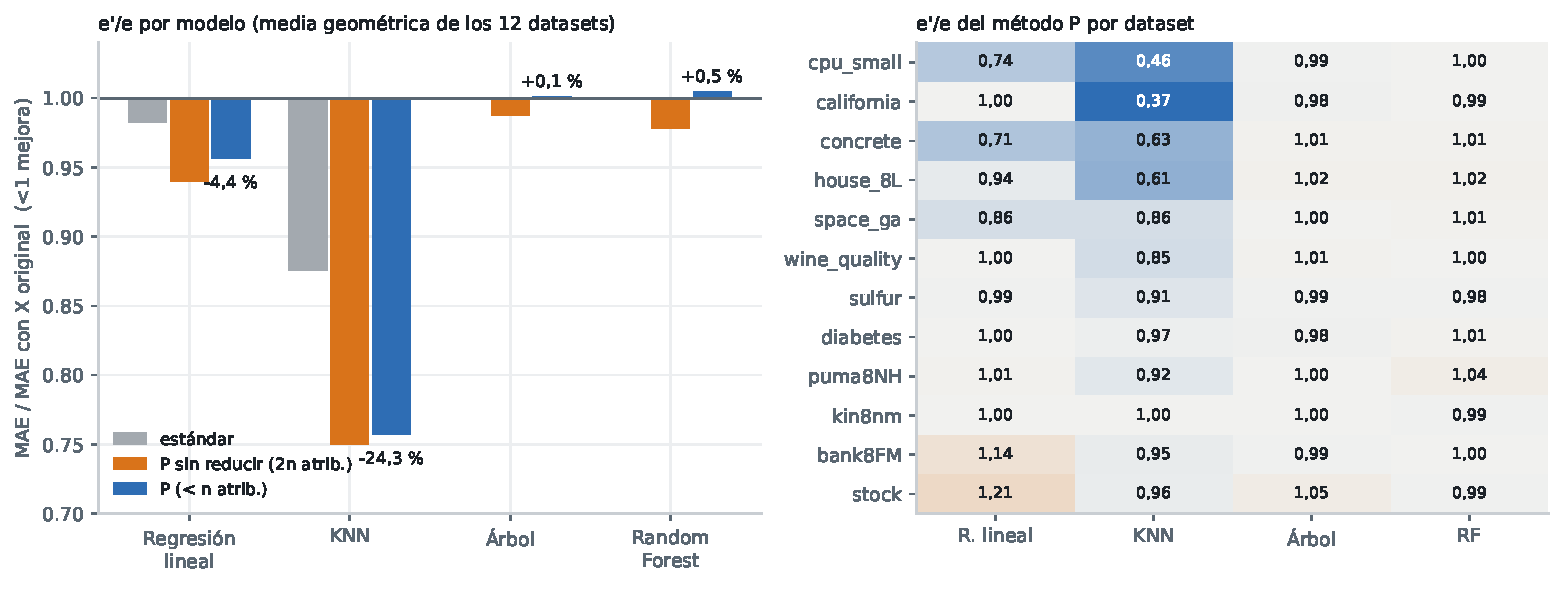
\includegraphics[width=0.86\textwidth]{principal}
\caption{Izquierda: $e'/e$ por modelo para $X$ estandarizado, $P$ sin reducir ($2n$ atributos) y $P$ ($<n$).
Derecha: $e'/e$ de $P$ por dataset (azul: mejora; naranja: empeora).}
\label{fig:principal}
\end{figure*}

\section{Protocolo}
Doce datasets de regresión: diabetes y california (práctica) y diez de OpenML (concrete, stock, space\_ga, sulfur,
kin8nm, bank8FM, puma8NH, house\_8L, cpu\_small, wine\_quality; 6--12 atributos, $\le$10\,000 filas). Las variantes
se exploraron con otras semillas; \textbf{todo lo que sigue usa particiones 70/30 nuevas} (semillas 40--44). La
ausencia de penalización por dimensión se fijó antes de ver estos resultados. \textbf{Modelos triviales y fijos}: RL,
KNN ($k=5$), árbol y Random Forest (100 árboles), con parámetros por defecto: el enunciado fija $M$.
\textbf{Estadística por dataset}: las particiones de un dataset comparten filas, así que la unidad es el dataset
(n=12), resumido con la media geométrica de $e'/e$; pares con Wilcoxon y corrección de Holm; comparaciones múltiples
con Friedman y Nemenyi (Demšar, 2006).

\section{Resultados}
\subsection{Criterio del enunciado}
\begin{table}[t]\centering\footnotesize\setlength{\tabcolsep}{2.4pt}
\caption{$e'/e$ (media geométrica de los 12 datasets). \emph{Datasets}: con $e'<e$; $p$: Wilcoxon por dataset con
Holm (8 contrastes); última columna: cambio de $P$ frente a $X$ estandarizado.}
\label{tab:principal}
\begin{tabular}{@{}lcccccc@{}}\toprule
Modelo & estándar & $P$ sin red.\ ($2n$) & $P$ ($<n$) & Datasets & $p$ & vs.\ est.\\\midrule
\filasPrincipal\bottomrule
\end{tabular}
\end{table}

Con $\dim X'<n$ (Tabla~\ref{tab:principal}, Fig.~\ref{fig:principal}), la mejora en KNN es grande y concluyente:
\cambioKNN{} frente a $X$ original ($p=$\pKNN, \dsKNN{} datasets) y \cambioVsEstKNN{} frente a estandarizar
($p=$\pVsEstKNN). En RL el error baja \cambioRL{} (\dsRL{} datasets), sin significación con 12 datasets y Holm; el
peor caso es stock (\peorDsRL). En el árbol (\cambioArbol) y en RF (\cambioRF) $P$ deja el error igual: \textbf{$e'<e$
solo se cumple en media para KNN y RL}.

\subsection{La reducción de dimensionalidad}
\begin{table}[t]\centering\footnotesize\setlength{\tabcolsep}{4pt}
\caption{Reducción aprendida (media de 5 particiones): $n$ atributos, $s$ conservados, $m$ componentes sintetizadas,
$\dim X'=s+m$ y umbral $\tau$ (mediana).}
\label{tab:dimension}
\begin{tabular}{@{}lccccc@{}}\toprule
Dataset & $n$ & $s$ & $m$ & $\dim X'$ & $\tau$\\\midrule
\filasDimension\bottomrule
\end{tabular}
\end{table}
$X'$ usa de media el \dimMedia{} de los atributos (entre \dimMin{} y \dimMax{} por partición) y siempre menos de $n$
(Tabla~\ref{tab:dimension}): la evolución elimina el \fracEliminados{} de los atributos originales, con un umbral
mediano $\tau=$\tauMediana. En la mayoría de datasets elimina uno o dos atributos; en puma8NH, donde solo unos pocos
atributos explican $y$, se queda con 2 y los complementa con componentes. \textbf{Qué cuesta reducir}: frente a $P$
sin reducir ($2n$ atributos), KNN cambia \cambioRedKNN{} ($p=$\pRedKNN), RL \cambioRedRL{} y el árbol
\cambioRedArbol, sin significación; RF empeora \cambioRedRF{} ($p=$\pRedRF, Holm), porque pierde las $n$ direcciones
oblicuas que le daba la síntesis completa. \textbf{Qué aporta la síntesis} dentro del presupuesto: CMA-ES solo
sintetiza en el \fracConSintesis{} de las particiones ($m=$\mMedia{} de media) y quitarla ($\rho=0$) apenas cambia
nada (RF \cambioSintRF, RL \cambioSintRL): con un fitness de KNN, el hueco liberado no se aprovecha para dar cortes
oblicuos. \textbf{Umbral fuera de la evolución}: aplicar a los $\theta$ de $P$ sin reducir una regla fija (quitar
atributos por peso creciente hasta el menor $s<n$ dentro de un error estándar del mejor fitness) da un resultado
parecido (KNN \cribSelKNN, RL \cribSelRL, RF \cribSelRF; \cribDimSel{} de los atributos); en cambio, un umbral fijo
$w_j<0{,}1$ no reduce nada en \cribFijoNoReduce{} particiones. Aprender $\tau$ dentro de la búsqueda cumple siempre
el enunciado sin añadir reglas externas.

\subsection{Comparativa con otras transformaciones}
En las mismas particiones comparamos $P$ con estandarizar, Yeo-Johnson por máxima verosimilitud
(\texttt{PowerTransformer}), cuantiles, ``solo PCA'' (sustituir $X$ por sus componentes con el 95\,\% de varianza o
con el \% elegido por validación cruzada, o añadirlas), aprendizaje de métricas para regresión (MLKR) y construcción
de atributos con programación genética (PG, \texttt{gplearn}: 500 individuos, 10 generaciones, $n$ atributos nuevos).
La Tabla~\ref{tab:comparativa} resume el resultado (Friedman: $p<0{,}001$ en los cuatro modelos). Las tres
transformaciones con mejor rango medio (\textbf{$P$ sin reducir}, \rangoPsr; estándar + su PCA y PG) usan $2n$
atributos. \textbf{Entre las que no aumentan la dimensión, $P$ es la mejor} (\rangoP, frente a \rangoYJMV{} de
Yeo-Johnson por máxima verosimilitud) y la única que reduce. En KNN supera a todas salvo a MLKR y a $P$ sin reducir
(sin diferencia significativa); en RL gana PG (\compPGRL{} frente a \compPRL, no significativo); en los árboles,
``solo PCA'', la otra forma de reducir, empeora mucho a RF (\compPCAnoventaRF): se pierden los ejes originales, que
suelen ser buenos cortes.

\begin{table}[t]\centering\footnotesize\setlength{\tabcolsep}{2.4pt}
\caption{Comparativa: $e'/e$ por modelo (negrita: mejor), $^*$: $P$ es mejor con $p<0{,}05$ (Wilcoxon por dataset,
Holm). Rango: medio de Friedman sobre los cuatro modelos (1 = mejor). $d/n$: $\dim X'$ relativa.}
\label{tab:comparativa}
\begin{tabular}{@{}lcccccc@{}}\toprule
Transformación & R.\ lin. & KNN & Árbol & RF & Rango & $d/n$\\\midrule
\filasComparativa\bottomrule
\end{tabular}
\end{table}

\subsection{La síntesis en los árboles}
\begin{figure}[t]\centering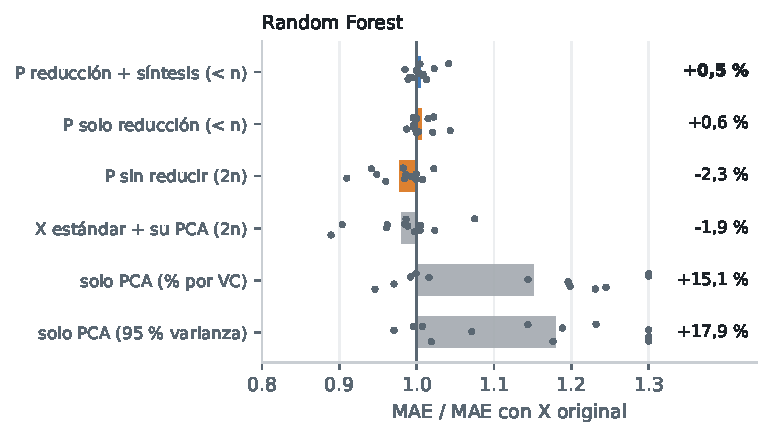
\includegraphics[width=\columnwidth]{sintesis_rf}
\caption{Variantes en las mismas particiones (Random Forest). Punto: dataset; barra: media geométrica.}
\label{fig:sintesis}
\end{figure}
La Fig.~\ref{fig:sintesis} resume la tensión. Lo que ayuda a RF es \emph{añadir} direcciones oblicuas a los ejes
originales ($P$ sin reducir \compPsrRF; $X$ estándar con su PCA \compEstPCARF), lo que exige $\dim X'>n$; sustituir
los ejes por componentes (``solo PCA'') lo empeora un 15--18\,\%. Con $\dim X'<n$, $P$ queda en \compPRF: no
empeora a RF, pero ya no lo mejora.

\subsection{La búsqueda: piezas, inicio, rango y algoritmo}\label{sec:busqueda}
\begin{table}[t]\centering\footnotesize\setlength{\tabcolsep}{4pt}
\caption{Ablación de la búsqueda de $(\lambda,w)$: cambio del MAE frente a CMA-ES ($m_0=\theta_0$, $\sigma_0=0{,}2$,
población por defecto, $\lambda\in[-2,2]$) en \nAblCasos{} particiones ($>0$: peor; $^*$: $p<0{,}05$ por dataset,
Holm).}
\label{tab:ablacion}
\begin{tabular}{@{}lccc@{}}\toprule
Variante & KNN & R.\ lineal & RF\\\midrule
\filasAblacion\bottomrule
\end{tabular}
\end{table}
La Tabla~\ref{tab:ablacion} cambia una sola decisión de la búsqueda de $(\lambda,w)$ cada vez (con $P$ sin reducir;
el $P$ final solo añade $\tau$ y $\rho$ al genoma). \textbf{Piezas}: los pesos son la pieza principal (quitar los
exponentes, $w=1$, empeora a KNN un \ctrlExp, $p=$\pCtrlExp), y en el $P$ final deciden además qué se elimina.
\textbf{Búsqueda}: la búsqueda aleatoria con el mismo presupuesto es \ctrlAleat{} peor en KNN ($p=$\pCtrlAleat), y
los pesos por información mutua, \ctrlMI. \textbf{Inicio}: CMA-ES es robusto a cómo empieza; mantenemos
$m_0=\theta_0$ porque arranca en la línea base y hace la búsqueda reproducible. \textbf{Rango}: ampliar $\lambda$ a
$[-4,4]$ u $[-8,8]$ tiende a empeorar sin significación; $[-2,2]$ evita el colapso numérico (el \mleFueraDos{} de los
$\lambda$ de máxima verosimilitud cae fuera). \textbf{Algoritmo} (Tabla~\ref{tab:algoritmos}): CMA-ES tiene el mejor
rango de fitness (\rangoCMA), pero las demás metaheurísticas quedan cerca y solo la búsqueda aleatoria es claramente
peor: la búsqueda importa; el algoritmo concreto, bastante menos.

\begin{table}[t]\centering\footnotesize\setlength{\tabcolsep}{4pt}
\caption{Optimizadores con el mismo $\theta=(\lambda,w)$, fitness y presupuesto (\nAlgCasos{} particiones): rango
medio de fitness (1 = mejor) y cambio del MAE frente a $X$ original.}
\label{tab:algoritmos}
\begin{tabular}{@{}lccc@{}}\toprule
Algoritmo & rango & KNN & R.\ lineal\\\midrule
\filasAlgoritmos\bottomrule
\end{tabular}
\end{table}

\subsection{Coste y caso negativo}
Una búsqueda de $P$ tarda \segMediana\,s de mediana (máx.\ \segMax\,s) por partición con 20 procesos en paralelo, una
sola vez por dataset; aplicar la transformación después es inmediato y, al tener $X'$ menos columnas, los modelos se
entrenan más rápido. Es un orden de magnitud más caro que MLKR (\segMLKR\,s) o PG (\segPG\,s). En diabetes (309 filas
de entrenamiento) la búsqueda mejora el fitness pero no la validación de forma fiable: sobreajuste al criterio de
búsqueda con pliegues de $\sim$60 filas.

\section{Conclusiones}
\begin{itemize}
\item \textbf{$P$ cumple las dos exigencias del enunciado}: $\dim X'<n$ siempre (\dimMedia{} de los atributos de
media) con un criterio de eliminación aprendido por CMA-ES, y síntesis de componentes cuando el fitness la elige.
\item \textbf{$e'<e$ en media para KNN} (\cambioKNN, concluyente) \textbf{y RL} (\cambioRL, no significativo); en los
árboles el error queda igual.
\item \textbf{Reducir y sintetizar compiten}: a los árboles les ayuda \emph{añadir} direcciones, lo que exige
aumentar la dimensión; con $\dim X'<n$ y un fitness de KNN la evolución prefiere quedarse con los atributos
originales. Reducir cuesta poco salvo en RF (\cambioRedRF).
\item \textbf{Entre las transformaciones que no aumentan la dimensión, $P$ tiene el mejor rango medio.}
\item \textbf{Límites}: 12 datasets numéricos y pequeños; sobreajuste con pocos datos; el fitness optimiza KNN; coste
de $\sim$3 minutos por búsqueda. Un fitness que combine varias familias de modelos podría repartir mejor el
presupuesto de atributos entre originales y componentes.
\end{itemize}

{\footnotesize\textbf{Reproducibilidad.} \texttt{reduccion/metodo\_reduccion.py} (programa $P$) y
\texttt{experimento\_reduccion.py}; \texttt{final/}: \texttt{metodo.py}, experimentos, \texttt{analisis.py} (tablas,
figuras y cifras) y \texttt{notebook\_final.ipynb} (todo el proceso, ejecutable).\par}
\end{document}
